\chapter{ TESTS}
Dans cette section nous présentons les tests unitaires et d'intégration réalisés sur les classes implémentées dans la partie Modèle. Dû à une contrainte de temps, nous n'avons pas pu réaliser de tests automatiques dit "end to end".  Nous avons tout de même testé manuellement les différentes fonctionnalités liées à l'interface, bien que cela ne soit pas suffisent.
\\
Les tests ont été lancés depuis Android studio en utilisant JUnit (version min 4.+). 

\subsection{Test classe FileManager}
La classe FileManager ne nécessite pas de beaucoup de tests unitaires puisqu'elle fait majoritairement appel à des fonctions liées à l'API Android (Bitmap, Matrix). 
Par conséquent nous avons eu besoin de tester les méthodes intToString, et getNextFragment.
Il est nécessaire de s'assurer du bon retour de getNextFragment puisque c'est grâce à cette méthode que l'on peut envoyer chaque partie de l'image, cela joue donc un rôle clé dans la futur reconstruction.

\begin{figure}[H]
    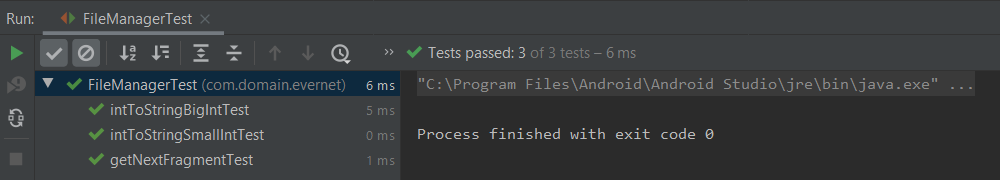
\includegraphics[width=18cm]{images/fileManagerOutput.png}
    \caption{Sortie de la classe de test FileManager.}
\end{figure}

\subsection{Test classe Client}
La classe Client joue un des rôles majeurs dans l'application Evernet, il est nécessaire de s'assurer de son bon fonctionnement. Nous avons donc testé la communication avec le serveur du groupe 1, c'est à dire l'ouverture, et la fermeture de sockets, ainsi que l'envoi et la réception de données. Il s'agit donc de la seule classe qui bénéficie de tests d'intégration puisque les tests font appel à la bibliothèque Java Socket qui n'est pas "mock".
\\
Cette classe nous a demandé le plus de travail en temps, puisque les tests d'intégration sont plus délicats à réaliser, en effet nous n'avons pas la main sur le serveur et la base de données, ce qui complexifie le processus. Nous avons donc réalisé ces tests avec le groupe 1 qui s'est tenu disponible pour nous aider à débugger lorsque nécessaire.
\\
\\
Deux tests unitaires sont réalisés permettant d'une part de vérifier le découpage correcte des réponses du serveur pour retirer les marqueurs de début et de fin, et d'autre part la construction d'une requête avec les marqueurs.
\begin{figure}[H]
    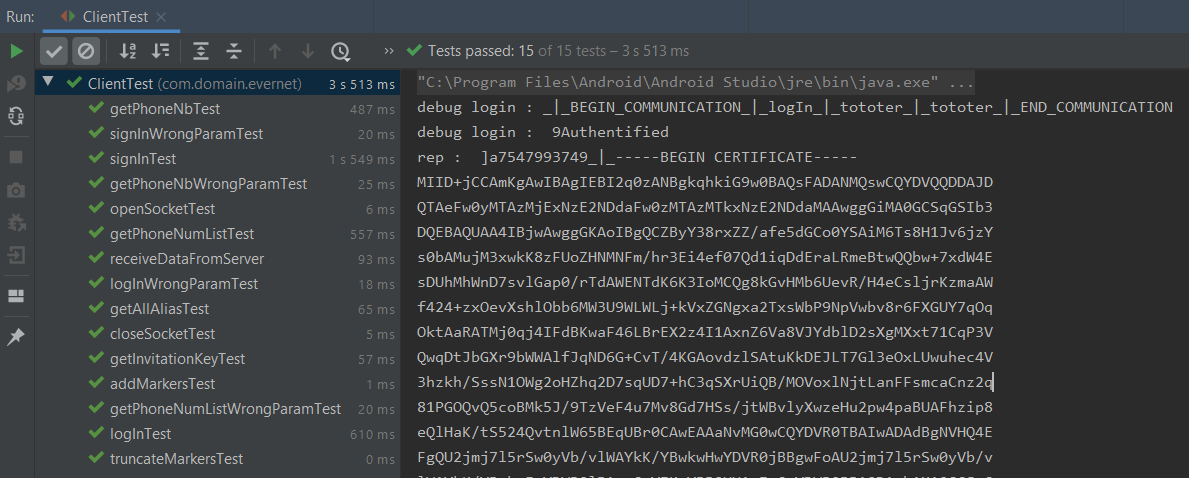
\includegraphics[width=18cm]{images/clientTestOutput.png}
    \caption{Sortie de la classe de test Packet.}
\end{figure}



\subsection{Test classe Packet}
La classe paquet est une autre classe majeure puisqu'elle joue un rôle clé dans le fonctionnement global du network coding. Il est donc très important de s'assurer que l'extraction de chaque champs d'un paquet est correctement réalisé. Nous avons également testé notre méthode permettant de générer un bourrage sur les champs concernés.

\begin{figure}[H]
    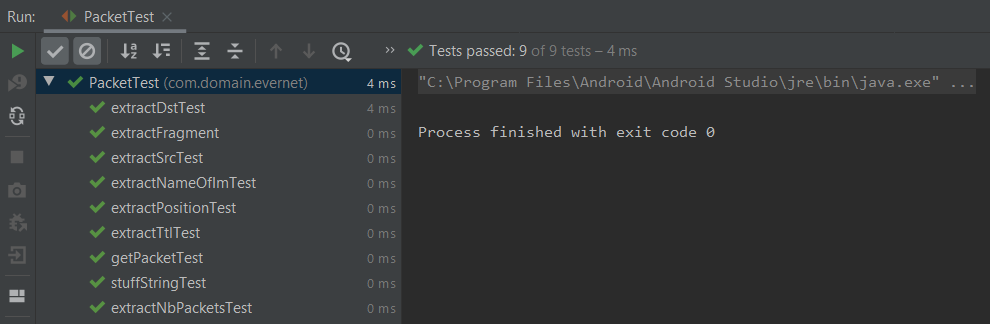
\includegraphics[width=18cm]{images/packetTestOutput.png}
    \caption{Sortie de la classe de test Packet.}
\end{figure}
